%!TEX root = main.tex
\chapter{Problem Elaboration}
\label{chap:problemelaboration}
%
% #### Problem elaboration
% Explain more about agile methods, why reflection is important, what are the challenges etc. Then we can discuss the scenarios.  
% Important to build an argumentation that justifies our focus, and since we develop a tool for use with github, our discussion should focus on the role of the artifact in the process(and the collaboration 
% around it). This part should be based on literature on agile software development and reflection. 
%
\label{problemelaboration}
In this chapter we will elaborate on our problem by defining our task and presenting our high level requirements.
We will also present our two main scenarios and the context of these. 

%### MIRROR reflection model
% What role do we see fpr the Computer-supported reflection model of MIRROR? Make use of the different phases of work/reflection and consider the support that can be provided in each step.  
% Model can be found: http://www.mirror-project.eu/showroom-a-publications/deliverables/174-d14model  
% Using the model should make it easier to further specify the scenarios.  Where to put this

\section{Problem Definition}
\label{problemdefinition}

To answer our research questions we will develop a web-tool aimed at software development teams adopting an agile process model. Most agile process models adopt reflection sessions, and it is for this purpose the tool is to be helpful. Using the tool at a daily basis, like described in Scenario 1 on page \pageref{scenario1}, allows for collection of fresh data and triggers reflection upon experiences connected to these data. These daily summaries are saved and can also be shared with the rest of the development team. In Scenario 2, these daily reflection notes can be reviewed individually and/or by the team in order to identify experiences over the whole iteration. The team can also use the shared notes to compare experiences and trigger discussion and reflection upon these. 
Most of these teams use some sort of a project tracker with project artifacts, like programming code, text documents etc. We have chosen to focus on GitHub, but the tool could be adapted to work with any version tracker that allows for data collection. The tool will collect relevant data from the project repository on GitHub without any action needed from the user to do so. The tool will then scaffold and present these data in order to allow users to revisit, share and reflect upon agile project experiences.
The experiences will be presented in several different ways like activity-graphs, mood-graphs and tagclouds. These will act as reflection triggers and help the users to reflect on their work. These experiences will be collected and made available for the users and/or the team later. The tool will be designed with reflection in mind, but the tool will also function as 
a tool that fits several scenarios and can be used by different groups of users. The tool also functions well on its own, and can be explored and provide data from experiences outside of the mentioned scenarios. Users can at any time look into a repository, a milestone or a single issue and the tool will provide data that is useful for recollecting experiences and providing a basis for reflection upon these. 
The tool will be evaluated with software development teams in a course at the Norwegian University of Science and Technology. We have worked out two main scenarios described below, that these groups will be evaluated against in order to answer our research questions, but as mentioned our goal is to develop the tool to be usable towards a wide range of other scenarios. 

\section{Reflection and technology}
The world wide web and modern technologies provides easy access to enormous amounts of information. This means that in order to learn, learners must be able to make sense of the information collected.  
In order to achieve this and make conscious decisions of how to use information, learners need to reflect on the information they collect. Reflection upon the process of solving problems is necessary to achieve a good result and to improve the ability to learn from experiences. When supporting learning with technology, this technology should promote these aspects within learning\cite{Lin1999}

The main goal is to provide technology that enables efficient information retrieval, and to provide scaffolds that support reflective thinking and problem solving. In our task this means utilizing collaborative learning experiences. 

\section{Reflection aspects}
TODO:
Which are the aspects it is important to reflect on(and what type of data is important to do it)
What type of reflection sessions are needed/advisable?
\subsection{Short term vs long term objectives}
Short term vs long term reflection objectives. 

\section{Scenarios}
\label{problemdefinition}

Based on related work, we have developed two scenarios to show what we want our tool to support in terms of collaborative reflection and learning. These two scenarios will provide a basis for the requirement elaboration and design choices in development of the tool. 
\\
At the Norwegian University of Science and Technology, NTNU, a group of students are taking the course IT2901 - Informatics Project II\footnotemark.
In the course, the focus is not only on the project itself, but also on the process the group steps through in order to reach their goal, including group roles, distribution of work etc. At the end of the course, students have to present a product report, with their project results, and a process report, with their project process results and experiences. In addition to this, groups participate in a retrospective workshop at the end of the course. In these three scenarios, our users are students and part of a group in the course , with age ranging from 22 and up to 28 years old.
\\
The group is going to work on a customer-driven project, using an agile methodic like scrum. The group will be using Github as a versioning-control system. During the project work the team will use Github to collect information. The PeacefulBanana tool can then be used to gather this information and present it in a scaffolded way mainly to be used in reflection sessions. Users can though, at any time go into the application and gather relevant data if they want to. This data will help the group to see trending issues and problems they have come upon in the process. Each member of the group will register as a user on the PeacefulBanana tool. The users will then be connected together as a group. 
\\
The two scenarios described in the next sections provides examples of how we envision the usage of the PeacefulBanana tool in three different settings. First as a individual tool on a daily basis, then as part of a team collaborative reflection session.
These two scenarios were developed early in the development process. The first scenario features using the tool at the end of each working day as inspired by [ref to the 5 minute daily reflection session]. The second scenario where in the end of each iteration there is a retrospective reflection session. 
\\

\footnotetext{Informatics Project II is a course where students from the Informatics education program is put together in groups working on different software development projects. Key objectives of this course are gaining practical experience in GROUP-ORIENTED software engineering for a customer, covering the whole life-cycle of a software project - \url{http://www.ntnu.edu/studies/courses/IT2901}}

\subsection{Scenario 1 - Individual use on a daily basis}
\label{scenario1}
In this scenario, our students will be using the tool on a daily basis at the end of each working day.

 When the students enter the web-app, they will get a notification with a prompt to do the daily status update.

\begin{figure}[h!]
\label{newnotification}
\centering
	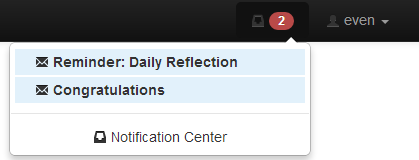
\includegraphics[width=\textwidth]{newnotification}
\caption{The user has clicked the notification icon and can see his new notifications}
\end{figure}

  When clicking the notification, the student is presented with a summary of their individual activity in the last 24 hours.
  This summary compares the commit activity of the user with the team's, and also presents a tagcloud representing the trending issues of the last day. The user is then prompted to input todays mood, their top two contributions \emph{"What did I do good?"} , and their top 2 points to improve on \emph{"What could I do better?"}. Finally the user can submit the form and choose to share these experiences with the team for collaborative use. The daily reflection notes are saved and can be reviewed at any time, and also shared any time by the user. The idea is that the tool will be used to revisit todays experiences with collected information presented in a way that triggers reflection upon these experiences. Information is collected and inspire new experiences. After working on a project that day, students "step back" to reflect on what happened during the day, and on the experiences they encountered. The tool provides scaffolded data to further trigger this reflection process. This process consist of returning to the experiences of that day, re-visit the experiences and attend to the feelings, like inputing todays mood. This reflection will help users to derive their top two improvements and contributions of the day\cite{Krogstie2011}. The tool thus captures the experiences and reflections made by the user and allows for re-visiting of these at a later date by storing them in the system. 

\subsection{Scenario 2 - Team use after each iteration}
\label{scenario2}
In this scenario, the students will be using the tool as part of the agile methodic two-week reflection sessions. Students will in this scenario use the tool to indicate how the project has been progressing over the last iteration, tightly coupled with one or several milestones. The students will generate tagclouds based on the trending issues in the relevant milestones, activity graphs and mood trajectories. Also if the users have chosen to share any of the individual reflection notes from scenario 1, these will be visible and can be used to draw conclusions from the previous iteration, and make comparisons. The tool will enable a group to see the whole iteration more clearly, but also be able to dive into certain issues or milestones that showed to be of particular interest, and thus create a discussion around the experiences made by the team members.  